\documentclass[a4paper,12pt, twoside, titlepage]{article}
\usepackage[utf8]{inputenc}
\usepackage{polski}
\usepackage[ddmmyyyy]{datetime}
\renewcommand{\dateseparator}{.}

\usepackage{lastpage}
\usepackage{fancyhdr}
\usepackage{graphicx}
\usepackage{hyperref}
\usepackage{longtable}
\usepackage{geometry}
\newgeometry{hmargin={20mm,20mm}, vmargin={30mm, 30mm}}


%\usepackage{hyperref}
%\hypersetup{
%    colorlinks,
%    citecolor=black,
%    filecolor=black,
%    linkcolor=black,
%    urlcolor=black
%}

%\renewcommand{\thesection}{\arabic{section}}

\pagestyle{fancy}
\fancyhf{}
\fancyhead[R]{\rightmark}
\fancyhead[L]{Eternal Fortification}
\fancyfoot[RO, LE]{\thepage \hspace{1pt} / \pageref{LastPage}}
\renewcommand{\footrulewidth}{0.5pt}

\renewcommand{\figurename}{Rysunek} 
\renewcommand{\sectionmark}[1]{\markright{#1}{}}

\title{\Huge{\textbf{Eternal Fortification}}\\ \Large{Projekt gry}\\ \large{Wersja 0.1}}
\author{Konrad Magiera}
\date{\today}


\begin{document}
\pagenumbering{gobble}
\maketitle
\newpage
\pagenumbering{arabic}
\tableofcontents
\newpage


\section{Przegląd}
\subsection{Gatunek}
Jest to strategiczna gra czasu rzeczywistego - Tower defense.

\subsection{Temat przewodni}
Gra porusza temat ewolucji, rozwoju cywilizacji. Kolejne poziomy wprowadzają gracza w następujące po sobie okresy rozwoju ludzkości.

\subsection{Opis projektu}


\subsection{Co wyróżnia projekt}
Pośród innych tytułów z gatunku Tower defense, Eternal Fortification wyróżnia motyw edukacyjny. Gra pozwala zapoznać się z uzbrojeniem wykorzystywanym przez ludzi na przestrzeni wieków.

\subsection{Dla kogo}
Idealnym odbiorcą będzie:
\begin{itemize}
	\item Osoba płci męskiej,
	\item Pasjonat historii,
	\item Osoba w wieku 15 - 24 lat.
\end{itemize}

\subsection{Użyta technologia}
Do stworzenia gry użyty zostanie silnik Unity3D oraz język C\#. Modele przygotowane zostaną w darmowym oprogramowaniu Blender.

\subsection{Wymagania systemowe}
\begin{itemize}
	\item System operacyjny: Windows 7/8.1.10,
	\item 1GB wolnego miejsca na dysku,
	\item 2GB RAM
\end{itemize}


\newpage
\section{Fabuła}
\subsection{hm}
\newpage
\section{Rozgrywka}
\subsection{Cel gry}
Gracz na każdym poziomie musi bronić się przed falami przeciwników. Warunkiem zwycięstwa jest przetrwanie określonej liczby fal dla danego poziomu. Liczba fal będzie różnić się pomiędzy poziomami podczas postępu w grze. Gracz przegrywa dany poziom gdy straci całe życia. Życia traci się gdy przeciwnicy dotrą do końca planszy.

\subsection{Tryb gry}
\subsubsection{Kampania}
Gracz z każdym zwycięstwem odblokowuje kolejne poziomy. W szczególnym przypadku odblokowana zostaje kolejna epoka, jeżeli wszystkie poziomy z danego okresu historycznego zostały ukończone. Kampania przenosi gracza w czasie, odkrywając kolejne okresy.

\subsection{Gracz}
\subsubsection{Sterowanie}
%\begin{figure}[!htb]
%		\begin{center}
%			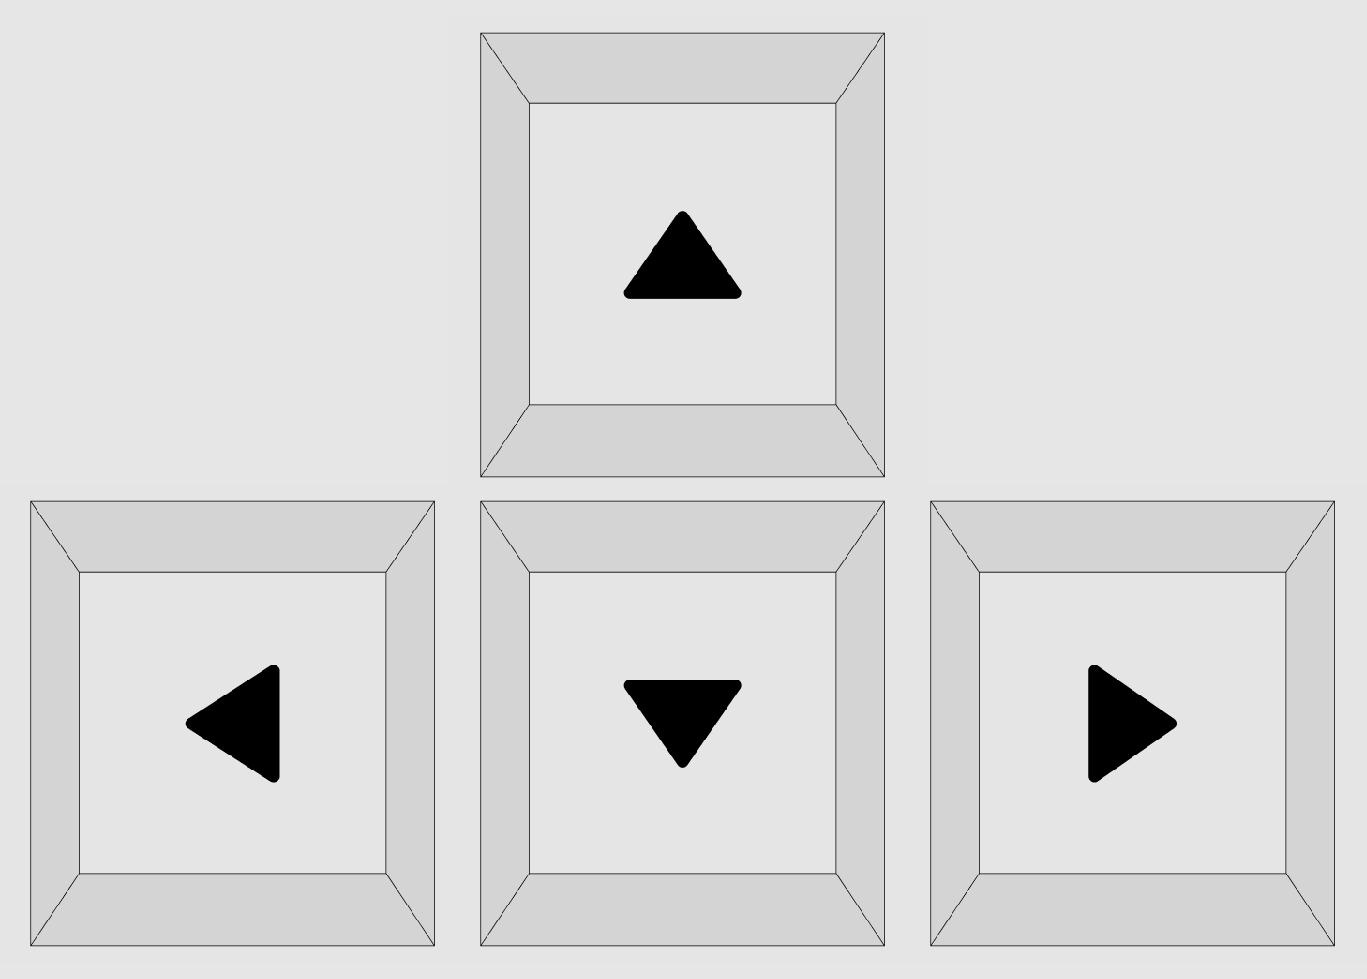
\includegraphics[height=3cm]{import/arrows.pdf}
%		\end{center}
%		\caption{Sterowanie}
%	\end{figure}

\begin{center}
\begin{longtable}{| p{.50\textwidth} | p{.50\textwidth} |} 
	\hline
	\begin{center}
		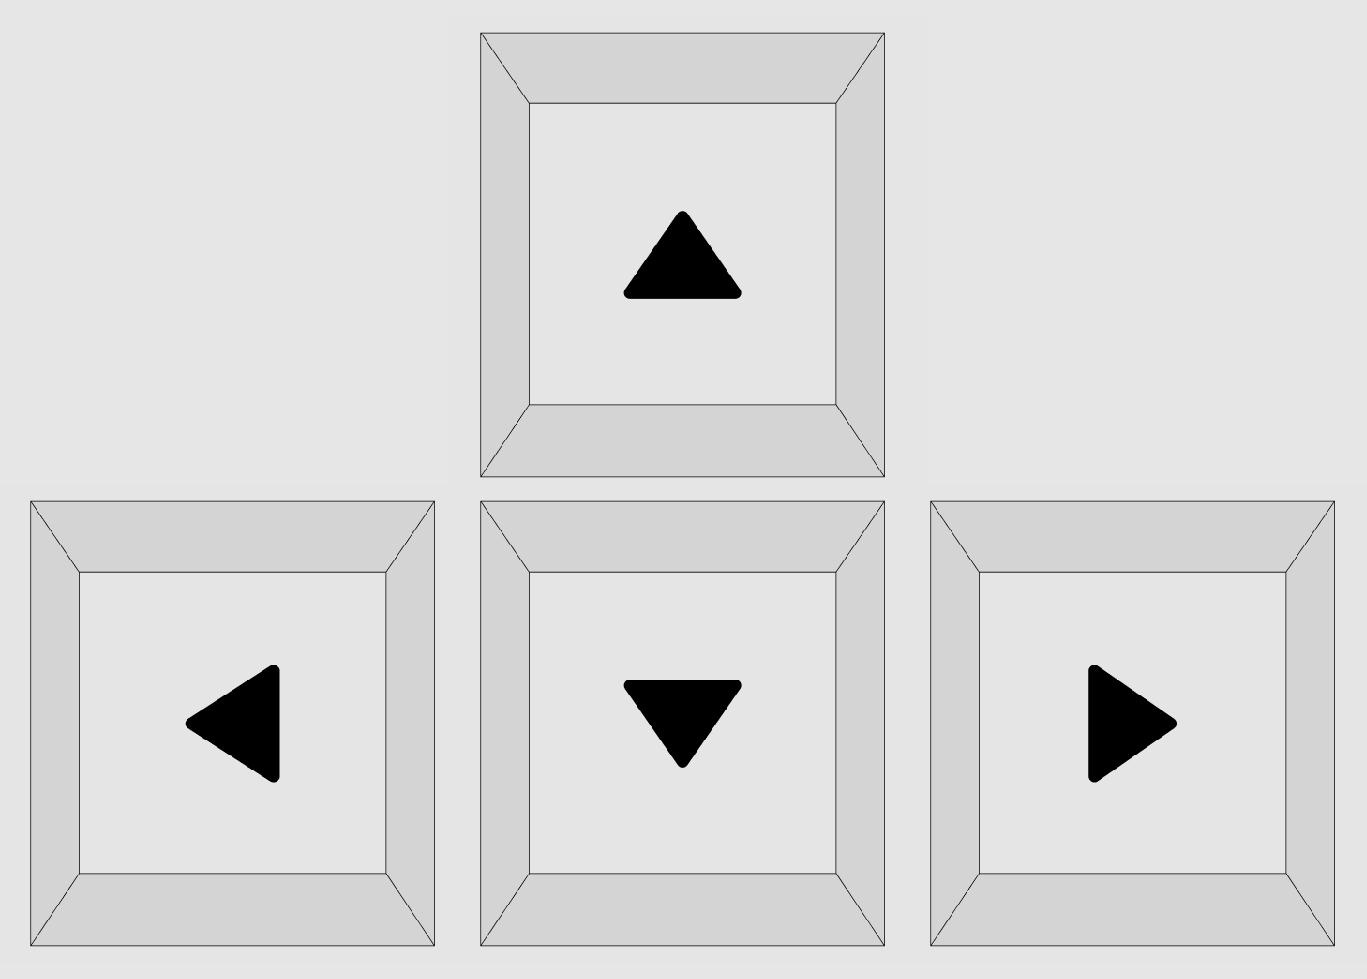
\includegraphics[height=3cm]{import/arrows.pdf}
	\end{center} 
	& Poruszanie kamerą na większych poziomach \\ 
	\hline 
	
	\begin{center}
		
\includegraphics[height=3cm]{import/mouse.pdf}
	\end{center}  & Pozostałe interakcje wykonywane przy pomocy myszki \\ 
	\hline
	

	\caption{Sterowanie}	
\end{longtable}
\end{center}

\subsubsection{Interfejs użytkownika}
\subsubsection{Interakcje}
\subsection{Przeciwnicy}
\subsubsection{Poruszanie}
\subsubsection{Statystyki}
\subsubsection{Okresy historyczne}
\subsection{Obrona}
\subsubsection{System celowania}
\subsubsection{Statystyki}
\subsubsection{Okresy historyczne}
 
\newpage
\section{Potrzebne materiały}
\subsection{Dźwięki}
\subsection{Modele}
\subsection{Efekty wizualne}
\subsection{Kod}
TMP
\cite{GDD-stanley}


\newpage
\section{Bibliografia}

\begingroup
\renewcommand{\section}[2]{}%
\begin{thebibliography}{}
\bibitem{GDD-stanley}
	Alec Markarian, Benjamin Stanley.
	\emph{Game Design Document}

	\href{https://docs.google.com/document/d/1-I08qX76DgSFyN1ByIGtPuqXh7bVKraHcNIA25tpAzE}{docs.google.com/document/d/1-I08qX76DgSFyN1ByIGtPuqXh7bVKraHcNIA25tpAzE}\\
	(dostęp 29.02.2020)

\bibitem{GDD}
	Chop Socky Chooks in Bantam Menace Game Design Document Version 1.1 Gas Ferry Rd, Bristol, BS1 6UN, \url{http://www.photonstorm.com/downloads/CSC_GDD.pdf}\\
	(dostęp 29.02.2020)

\end{thebibliography}
\endgroup

\end{document}

